\maketitle

\section*{Overview}\label{sec:overview}
EduSoC (Educational System on Chip) is an FPGA-based, RISC-V-oriented system-on-chip infrastructure.
It is designed for educational purposes, offering minimal complexity and consisting of a small set of essential modules and peripherals:
\begin{itemize}
    \item Clock and reset signal generation
    \item Boot ROM (size and speed configurable)
    \item Block RAM (size and speed configurable)
    \item SoC controller with interrupt engine supporting up to 32 interrupts
    \item GPIO module with change notification interrupt, supporting up to 512 GPIO pins
    \item Timer module with up to 16 independent timers with configurable periods and interrupts
    \item PWM module with up to 16 independent pulse width modulated outputs
    \item VGA controller with 8-bit color framebuffer (size and speed configurable)
    \item Serial UART bridge for external memory programming and SoC/peripheral control
    \item Crossbar bus interconnect
\end{itemize}
In its default configuration, EduSoC is intended for use with a Digilent Arty S7 board and offers a Verilog-compatible module for use with this board (\ttt{edusoc\_basic}, see Appendix \ref{sec:basic}). However, EduSoC can be configured for any hardware platform, and more peripherals can be added to EduSoC with relative ease.

EduSoC does not target or contain any specific RISC-V core. A simple core interface is provided.

\newpage
\tableofcontents
\listoffigures
\listoftables
\newpage

\section{System Structure}\label{sec:structure}
\begin{figure}[H]
    \centering
    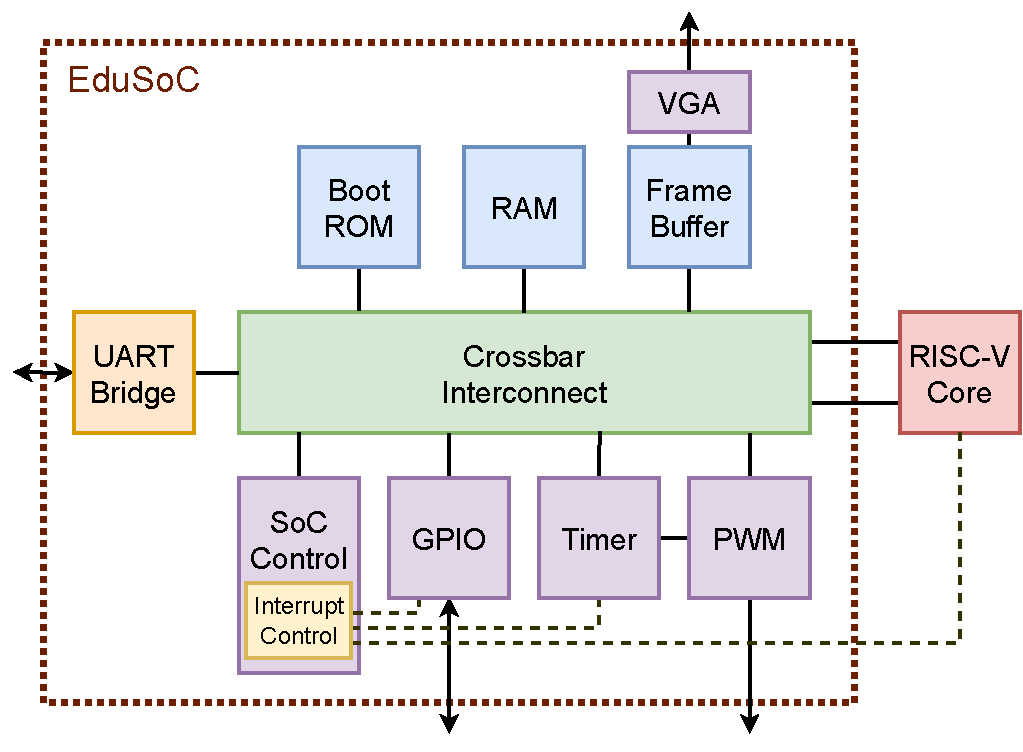
\includegraphics[width=\textwidth]{graphics/EduSoC Block Diagram.pdf}
    \vspace{-2em}
    \caption{System Block Diagram}
    \label{fig:block_diagram}
\end{figure}
EduSoC provides all components within the dotted frame. 

At its center, the crossbar interconnect serves as a bus connection between all system components.
The interconnect arbitrates three bus masters (the UART bridge and the core's data and instruction buses), where the UART bridge has priority over the other two.
The remaining SoC modules are bus slaves.

\newpage
\section{Memory Map}\label{sec:memorymap}
\begin{figure}[H]
    \centering
    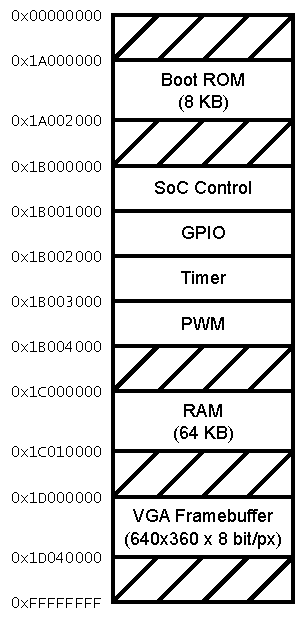
\includegraphics[height=.6\paperheight]{graphics/EduSoC Memory Map.pdf}
    \caption{Default Memory Map}
    \label{fig:memory_map}
\end{figure}
The above memory map represents the default configuration of EduSoC, and is fully configurable (see Section \ref{sec:config}).

Hatched areas are unused. Writing to them has no effect, and reading from them produces undefined values.